% Block layout: columns are stored separately, and the footer is what makes
% skipping possible.
\definecolor{accent}{HTML}{2F6FEB}
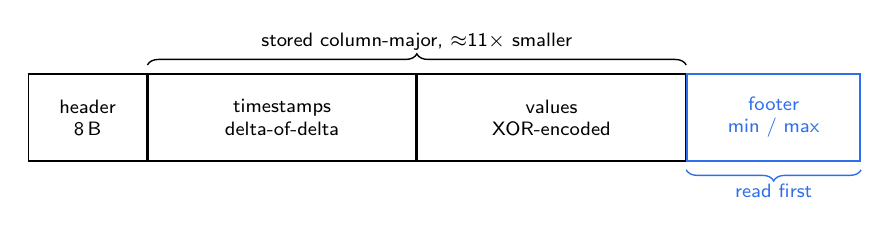
\begin{tikzpicture}[
  font=\small\sffamily,
  cell/.style={draw, line width=.6pt, minimum height=11mm, inner sep=3pt,
               font=\scriptsize\sffamily, align=center},
  lbl/.style={font=\scriptsize\sffamily, inner sep=2pt},
]
  \node[cell, minimum width=15mm] (hdr) at (0,0) {header\\8\,B};
  \node[cell, minimum width=34mm, anchor=west] (ts) at (hdr.east) {timestamps\\delta-of-delta};
  \node[cell, minimum width=34mm, anchor=west] (val) at (ts.east) {values\\XOR-encoded};
  \node[cell, minimum width=22mm, anchor=west, draw=accent, text=accent] (ftr) at (val.east)
        {footer\\min / max};

  \draw[decorate, decoration={brace, amplitude=4pt, raise=3pt}, line width=.5pt]
        (ts.north west) -- (val.north east)
        node[lbl, midway, above=6pt] {stored column-major, $\approx$11$\times$ smaller};

  \draw[decorate, decoration={brace, amplitude=4pt, raise=3pt, mirror}, line width=.5pt, draw=accent]
        (ftr.south west) -- (ftr.south east)
        node[lbl, midway, below=6pt, text=accent, align=center] {read first};
\end{tikzpicture}
